
\documentclass{amsart}


\usepackage{tikz}
\usepackage{tkz-berge}
\usepackage{mathpazo}
\title{MAS341 Practice Week 2}

\begin{document}



Hamilton marketed an ``icosian game'', whose object was to find Hamiltonian cycles on various graphs.  The base graph was the vertices an edges of a dodecahedron (as pictured below).  Find a Hamiltonian cycle for that graph. 

 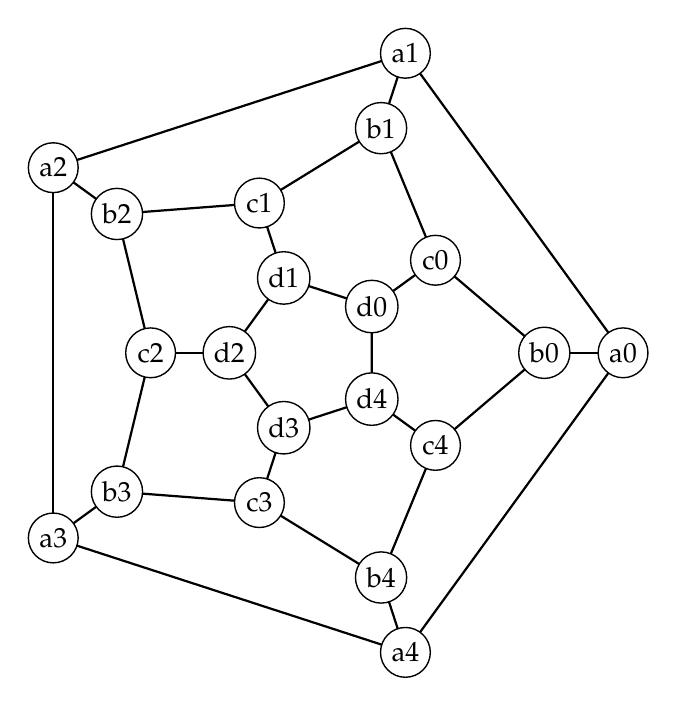
\begin{tikzpicture}
        \grDodecahedral[form=2] 
    \end{tikzpicture}
Prove that if we delete one vertex from this graph (say, a1) and the three edges adjacent to the vertex, the resulting graph with 19 vertices does \emph{not} have a Hamiltonian cycle (some case by case analysis is needed).


\end{document}
